\section{Comparison and takeaways}

\begin{frame}{Comparison: L0 vs L1/2 vs L1}
\small
\begin{tabularx}{\textwidth}{lXXX}
\toprule
 & \textbf{L0} & \textbf{L1/2} & \textbf{L1} \\
\midrule
Sparsity strength & Very high (ideal) & High & Medium/High \\
Convex? & No (discrete) & No ($p<1$) & Yes \\
Optimization & Hard (combinatorial) & Hard/medium (non-convex) & Easier (convex) \\
Stability & Can be unstable & Depends on solver/init & Usually stable \\
Typical use-cases & Strict subset selection & Need more sparsity than L1 & Strong baseline, interpretable \\
\bottomrule
\end{tabularx}
\end{frame}

\begin{frame}{When to use what?}
\begin{columns}[T,onlytextwidth]
  \begin{column}{0.33\textwidth}
    \begin{block}{Use L1}
      \begin{itemize}
        \item Convex + reliable
        \item Good baseline
        \item Fast training
      \end{itemize}
    \end{block}
  \end{column}
  \begin{column}{0.34\textwidth}
    \begin{block}{Use L1/2}
      \begin{itemize}
        \item Need stronger sparsity
        \item Accept non-convexity
        \item Careful optimization
      \end{itemize}
    \end{block}
  \end{column}
  \begin{column}{0.33\textwidth}
    \begin{block}{Use L0}
      \begin{itemize}
        \item Strict feature subset
        \item Manageable $p$
        \item Specialized solvers
      \end{itemize}
    \end{block}
  \end{column}
\end{columns}
\end{frame}

\begin{frame}{Conclusion}
\begin{itemize}
  \item \textbf{L0:} direct sparsity objective, very interpretable, but computationally hard.
  \item \textbf{L1/2:} a bridge between L0 and L1; often yields stronger sparsity than L1, but non-convex.
  \item Always balance: \textbf{accuracy} vs \textbf{sparsity} vs \textbf{compute}.
\end{itemize}

\vspace{0.8em}
\centering
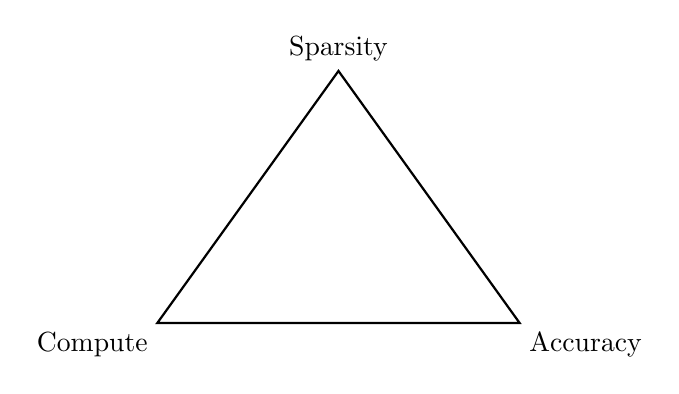
\begin{tikzpicture}[scale=1.0]
  \coordinate (A) at (0,0);
  \coordinate (B) at (4.6,0);
  \coordinate (C) at (2.3,3.2);
  \draw[thick] (A) -- (B) -- (C) -- cycle;
  \node[below left] at (A) {Compute};
  \node[below right] at (B) {Accuracy};
  \node[above] at (C) {Sparsity};
\end{tikzpicture}
\end{frame}

\begin{frame}{References (minimal)}
\small
\begin{itemize}
  \item Course notes / lecture slides on regularization and sparse modeling.
  \item Best subset selection / L0 regularization: classic regression model selection literature.
  \item Non-convex sparse penalties ($L_p$ with $p<1$): overview papers on non-convex regularization (optional).
\end{itemize}
\end{frame}